%label:"fig:fundamentalPolygonsT2"
%author:JeffHicks
%name:"fundamental polygons for $T^2$"
%type:"figure"
%caption:"There are many different fundamental polygons which represent the same surface."


\usetikzlibrary{decorations.markings}


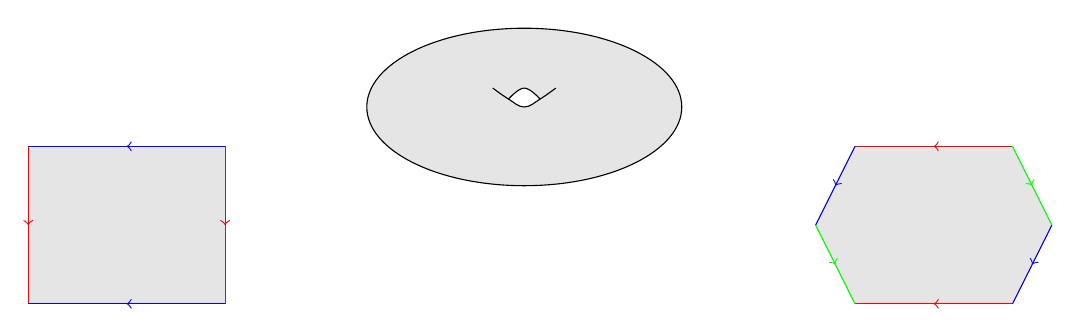
\begin{tikzpicture}
\tikzset{ ->-/.style={decoration={markings, mark=at position .5 with {\arrow{>}}}, postaction={decorate}}}
\draw[fill=gray!20]  (-1.2,-0.5) ellipse (2 and 1);

 \begin{scope}[shift={(2.2,-0.6)}]
    
    \fill[white]  plot[smooth, tension=0.7] coordinates { (-3.6,0.2) (-3.4,0.1) (-3.2,0.2) }  plot[smooth, tension=0.7] coordinates {(-3.6,0.2) (-3.4,0.34) (-3.2,0.2)};
    
    \draw  plot[smooth, tension=0.7] coordinates {(-3.8,0.34) (-3.6,0.2) (-3.4,0.1) (-3.2,0.2) (-3,0.34)};
    \draw  plot[smooth, tension=0.7] coordinates {(-3.6,0.2) (-3.4,0.34) (-3.2,0.2)};
    
    
    
    \end{scope}

\fill[gray!20]  (-7.5,-1) rectangle (-5,-3);
\fill[gray!20] (3,-1) -- (2.5,-2) -- (3,-3) -- (5,-3) -- (5.5,-2) -- (5,-1) -- cycle;

\draw[->-, red] (-5,-1) -- (-5,-3);
\draw[->-,red](-7.5,-1) -- (-7.5,-3);
\draw[->-, blue] (-5,-1) -- (-7.5,-1);
\draw[->-,blue] (-5,-3) -- (-7.5,-3);
\draw[->-, red] (5,-1) -- (3,-1);
\draw[->-,red] (5,-3) -- (3,-3);
\draw[->-,blue] (3,-1) -- (2.5,-2);
\draw[->-,blue] (5.5,-2) -- (5,-3);
\draw[->-,green] (5,-1) -- (5.5,-2);
\draw[->-,green] (2.5,-2) -- (3,-3);
\end{tikzpicture}